\documentclass[times, utf8, numeric]{beamer}
\usepackage[T1]{fontenc}

\renewcommand{\figurename}{Slika}
\setbeamertemplate{caption}[numbered]

\usetheme{Pittsburgh}
\usecolortheme{beaver}

\title{Razvoj podatkovnog sloja i aplikacijske logike za potrebe sustava elektroničkog učenja}
\subtitle{Završni rad, ak. god. 2015/16.}
\author{Alen Murtić
	\newline mentor: Doc. dr. sc. Damir Pintar}
\institute{Faklutet elektrotehnike i računarstva, Sveučilište u Zagrebu}
\date{04.07.2016.}

\begin{document}

\begin{frame}
	\titlepage
\end{frame}

\begin{frame}
	\frametitle{Sadržaj}
	\tableofcontents
\end{frame}

\section{Sustavi za elektroničko učenje}

\begin{frame}{Sustavi za elektroničko učenje}
	\begin{itemize}
		\item prijenos znanja ili obrazovnog programa putem elektroničkih uređaja
		\item prenošenje informacija i materijala, provjeravanje znanja, upijanje novih činjenica
		\item cilj: objedinjavanje procesa učenja
		\item prednosti: objektivnost, dostupnost (vremenska i lokacijska)
		\item nedostatak: mala individualnost
	\end{itemize}
\end{frame}

\subsection{Inteligentni sustavi za učenje (ITS)}
\begin{frame}{Inteligentni sustavi za učenje (ITS)}
\begin{itemize}
	\item J. Carbonell: \textit{"Sustav za učenje nije samo alat, nego i učitelj."}
	\item individualni pristup svakom korisniku, s obzirom na njegovo znanje i sposobnosti
	\item mogućnosti koje ITS treba nuditi:
	\begin{itemize}
		\item procjena korisnikova znanja
		\item inteligentno posluživanje pitanja
		\item reakcije i pomoć korisniku
	\end{itemize}
	\item reprezentacija znanje je iznimno važna za kvalitetu ITS-a
\end{itemize}
\end{frame}

\begin{frame}{Komponente ITS-a}
\begin{itemize}
	\item \textbf{domenski model}
	\begin{itemize}
		\item organizacija znanja u jedinice za pohranu u bazu podataka
		\item uključuje i strategije koje korisnik treba naučiti
	\end{itemize}
	\item \textbf{korisnički (učenički) model}
	\begin{itemize}
		\item evaluacija točnosti odgovora i analiza zadataka korak po korak
	\end{itemize}
	\item \textbf{model učenja}
	\begin{itemize}
		\item procjena i bodovanje korisnikova znanja, navigacija sustavom
	\end{itemize}
	\item \textbf{korisničko sučelje}
	\begin{itemize}
		\item grafički ili tekstualni način komunikacije s korisnikom
	\end{itemize}
\end{itemize}
\end{frame}

\section{Implementirano rješenje}
\begin{frame}{Implementirano rješenje}
zadatak završnog rada:
\begin{itemize}
	\item podatkovni sloj i aplikacijska logika ITS-a
	\item procjena i reprezentacija stanja usvojenosti koncepata
	\item baza parametriziranih zadataka
	\item inteligentno posluživanje zadataka
	\item sastavljanje ispita s obzirom na uvjete
\end{itemize}
\end{frame}

\subsection{Baza podataka}

\begin{frame}{ER dijagram}
\begin{figure}[er]
	\centering
	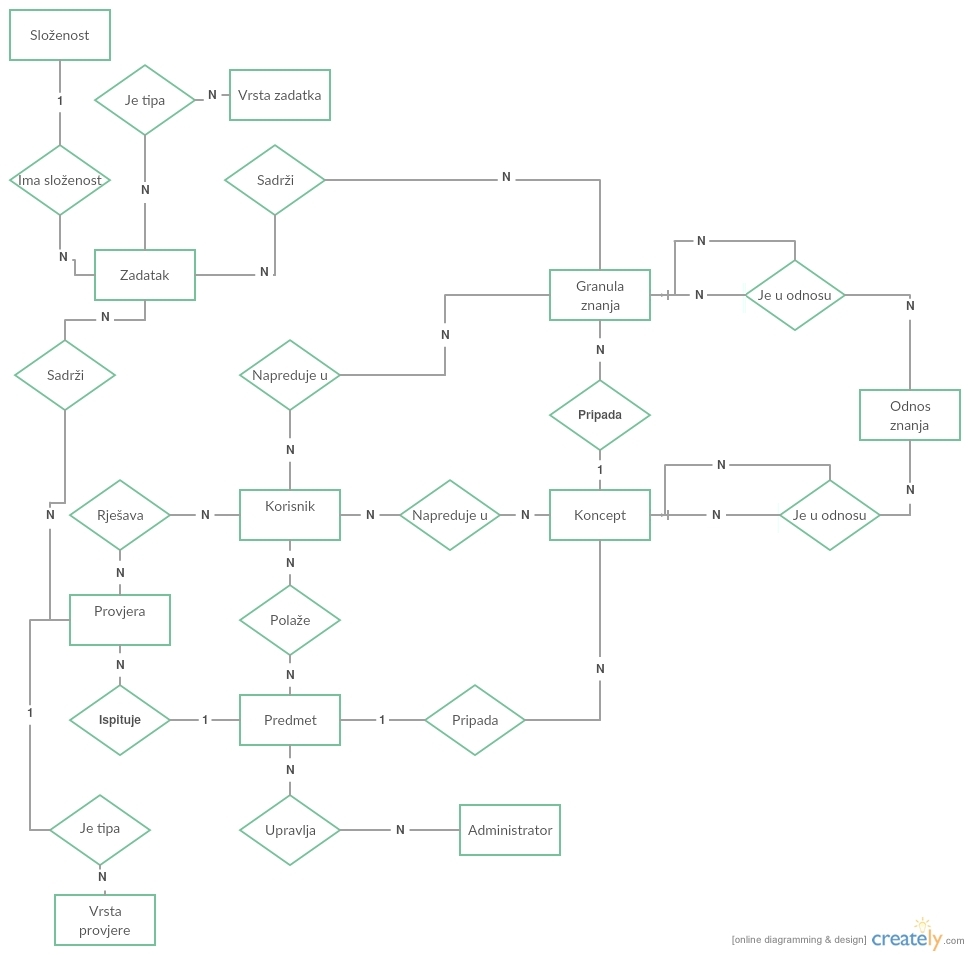
\includegraphics[width=\textwidth,height=0.7\textheight,keepaspectratio]{img/ER.jpg}
	\caption{ER dijagram baze}
	\label{fig:ER}
\end{figure}
\end{frame}

\begin{frame}{Baza znanja}
\begin{itemize}
	\item podjela znanja u granulacije:
	\begin{itemize}
		\item \textbf{predmet}
		\item \textbf{koncept} - pripada predmetu
		\item \textbf{granula} znanja - pripada konceptu
	\end{itemize}
	\item između dvaju koncepata ili granula mogući su odnosi:
	\begin{itemize}
		\item \textbf{preduvjet} - nemoguće je znati jedno bez znanja drugog
		\item \textbf{podskup} (nadskup) - jedna granulacije u cijelosti sadrži drugu
		\item \textbf{korištenje} - da bi se riješila pitanja neke granulacije, potrebno je koristiti znanje druge
		\item \textbf{analogno} - znanjem nečega postoji osnovno razumijevanje nečeg drugog
		\item \textbf{paralelno} - više pogleda na jedan problem
	\end{itemize}
	\item odnosi ne ovise o pripadnosti granulacije višoj, npr. mogući su odnosi između koncepata različitih predmeta
\end{itemize}
\end{frame}

\begin{frame}{Parametrizirana pitanja}
\begin{itemize}
	\item entitet zadatak u bazi opisuju atributi:
	\begin{itemize}
		\item pitanje - tekstualni opis
		\item slika - dodatak opis, neobavezna
		\item parametri - brojevi koji se generiraju prilikom stvaranja konkretnog pitanja, moguće definirati min. i max. vrijednost
		\item izraz - matematička formula za izračun rezultata konkretnih parametara
		\item složenost - težina pitanja (nije bitna za parametrizaciju)
		\item granula kojoj pripada (nije bitno za parametrizaciju)
	\end{itemize}
	\item korisniku se prikazuju pitanje, slika i konkretni parametri
	\item korisnikovo rješenje uspoređuje se s 5\% točnosti u odnosu na izračunato
\end{itemize}
\end{frame}

\subsection{Aplikacijska logika}
\begin{frame}{Procjena znanja korisnika}
\begin{itemize}
	\item granule
	\begin{itemize}
		\item korisnikovo znanje granule počinje od 0
		\item granuli pitanja i granuli nadskupa dodaje se ili oduzima faktor važnosti * broj složenosti granule za svaki zadatak
		\item granula ima upisanu svoju ukupnu bodovnu složenost u bazi
		\item faktor važnosti granule kojoj zadatak pripada i granule podskupa je 1, korištene granule 0.4, a analogne 0.2
	\end{itemize}
	\item koncepti
	\begin{itemize}
		\item težinski prosjek usvojenosti granula koje pripadaju konceptu
		\item težina granule je 5 * faktor važnosti
		\item računa se samo usvojenost granula koje pripadaju konceptu i povezanim konceptima
		\item težine su analogne težinama granula
	\end{itemize}
\end{itemize}
\end{frame}

\begin{frame}{Znanje u sustavu}

\begin{itemize}
	\item diskretna matematika
	\begin{itemize}
		\item osnove kombinatorike
		\begin{itemize}
			\item skupovi, produktno pravilo, permutacije
		\end{itemize}
		\item varijacije i kombinacije
		\begin{itemize}
			\item varijacije, kombinacije
		\end{itemize}
	\item napredna kombinatorika
	\begin{itemize}
		\item mješovita kombinatorika, Dirichletovo načelo
	\end{itemize}
	\item osnove vjerojatnosti
	\begin{itemize}
		\item osnove vjerojatnosti
	\end{itemize}
\end{itemize}
	\end{itemize}
\end{frame}

\begin{frame}{Generiranje pitanja}
\begin{itemize}
	\item inteligentno učenje - algoritam:
	\begin{enumerate}
		\item odabir koncepata koje korisnik može odgovarati
		\item odabir svih dostupnih granula znanja unutar koncepata
		\item permutacija liste granula i lista pitanja svake granule
		\item pronalazak po jednog pitanja složenosti najsličnije korisnikovu znanju za svaku granulu
		\item ako nema dovoljno pitanja, povećanje broja pitanja za 1 po granuli dok se na nađe dovoljno
	\end{enumerate}
	\item s obzirom na uvjete administratora (ispit)
	\begin{itemize}
		\item odabir minimalne i maksimalne moguće složenosti pitanja
		\item odabir korisnika kojemu se ispit generira
		\item upozorenje ako neki korisnik ne smije dobiti neka pitanja
		\item inteligentan odabir za svakog korisnika
	\end{itemize}
\end{itemize}
\end{frame}

\section{Pitanja}
\begin{frame}{Pitanja}
	\begin{figure}[pitanja]
		\centering
		
\includegraphics[width=\textwidth,height=0.7\textheight,keepaspectratio]{img/pitanja.png}
		%\caption{ER dijagram baze}
		\label{fig:ER}
	\end{figure}
\end{frame}

\section{Literatura}
\begin{frame}{Literatura}
\begin{itemize}
	\item D. Stockley. E-learning definition (elearning, online training, online learning).
	http://www.derekstockley.com.au/elearning-definition.html. Preuzeto: 3. 7. 2016.
	\item
	M. Urban-Lurain. Intelligent tutoring systems: An historic review in the context
	of the development of artificial intelligence and educational psychology.
	http://www.cse.msu.edu/rgroups/cse101/ITS/its.htm. Preuzeto: 3. 7. 2016.
\end{itemize}
\end{frame}

\end{document}